\chapter{SYSTEM DESIGN}



\section{Use case model}

\begin{figure}[H]
    \centering
    \begin{tikzpicture}[
        usecase/.style={draw=blue!60, fill=blue!8, shape=ellipse, minimum width=4.2cm, minimum height=0.85cm, align=center, font=\scriptsize},
        rel/.style={-Latex, thick, gray!70}
    ]

    % System boundary
    \draw[rounded corners=6pt, thick, gray!50] (-4.8,4.2) rectangle (4.8,-7.8);
    \node[font=\small\bfseries] at (0,4.5) {Smart Price-to-Quality Product Advisor System};

    % User use cases (left side)
    \node[usecase] (u_register)  at (0,3.4)  {Register and Login};
    \node[usecase] (u_browse)    at (0,2.2)  {Browse Available Products};
    \node[usecase] (u_search)    at (0,1.0)  {Search and Filter Products};
    \node[usecase] (u_details)   at (0,-0.2) {View Product Details};
    \node[usecase] (u_compare)   at (0,-1.4) {Compare Products};
    \node[usecase] (u_recommend) at (0,-2.6) {View Recommendations};
    \node[usecase] (u_wishlist)  at (0,-3.8) {Manage Wishlist};

    % Admin use cases (lower)
    \node[usecase] (a_login)  at (0,-5.0) {Admin Login};
    \node[usecase] (a_add)    at (-2.2,-6.3) {Add Products};
    \node[usecase] (a_update) at (0,-6.3)    {Update Products};
    \node[usecase] (a_delete) at (2.2,-6.3)  {Delete Products};
    \node[usecase] (a_manage) at (0,-7.3)    {Manage System Data};

    % ---- User stickman (left) ----
    \draw[thick] (-7.0,1.2) circle (0.25);
    \draw[thick] (-7.0,0.95) -- (-7.0,0.15);
    \draw[thick] (-7.35,0.65) -- (-6.65,0.65);
    \draw[thick] (-7.0,0.15) -- (-7.25,-0.35);
    \draw[thick] (-7.0,0.15) -- (-6.75,-0.35);
    \node[font=\small\bfseries] at (-7.0,-0.7) {User};

    % ---- Admin stickman (right) ----
    \draw[thick] (7.0,-4.8) circle (0.25);
    \draw[thick] (7.0,-5.05) -- (7.0,-5.85);
    \draw[thick] (6.65,-5.35) -- (7.35,-5.35);
    \draw[thick] (7.0,-5.85) -- (6.75,-6.35);
    \draw[thick] (7.0,-5.85) -- (7.25,-6.35);
    \node[font=\small\bfseries] at (7.0,-6.7) {Admin};

    % User relations (fan out from user body)
    \draw[rel] (-6.65,0.65) -- (u_register.west);
    \draw[rel] (-6.65,0.65) -- (u_browse.west);
    \draw[rel] (-6.65,0.65) -- (u_search.west);
    \draw[rel] (-6.65,0.65) -- (u_details.west);
    \draw[rel] (-6.65,0.65) -- (u_compare.west);
    \draw[rel] (-6.65,0.65) -- (u_recommend.west);
    \draw[rel] (-6.65,0.65) -- (u_wishlist.west);

    % Admin relations (fan out from admin body)
    \draw[rel] (6.65,-5.35) -- (a_login.east);
    \draw[rel] (6.65,-5.35) -- (a_add.east);
    \draw[rel] (6.65,-5.35) -- (a_update.east);
    \draw[rel] (6.65,-5.35) -- (a_delete.east);
    \draw[rel] (6.65,-5.35) -- (a_manage.east);

    \end{tikzpicture}
    \caption{Use Case Diagram for Smart Price-to-Quality Product Advisor System}
    \label{fig:use_case}
\end{figure}

\subsection{Actors and Roles}

The system involves two primary actors: \textbf{User} and \textbf{Admin}.

\textbf{Actor Name: User}

Role:
\begin{itemize}
\item Register and log in to the system
\item Browse available products
\item Search and filter products based on preferences
\item View detailed product information
\item Compare products side by side
\item View price-to-quality recommendations
\item Add or remove products from wishlist
\item Logout from the system
\end{itemize}

\textbf{Actor Name: Admin}

Role:
\begin{itemize}
\item Log in to the admin panel
\item Add new products to the database
\item Update existing product details
\item Delete products from the system
\item Manage and maintain product information
\item Monitor system data
\item Logout from the system
\end{itemize}

% =====================================================

\section{Activity Diagram (System Workflow)}

\begin{figure}[H]
    \centering
    \begin{tikzpicture}[
        node distance=0.85cm,
        act/.style={rectangle, rounded corners=4pt, draw=blue!55, fill=blue!8, minimum width=5.2cm, minimum height=0.75cm, align=center, font=\scriptsize},
        decision/.style={diamond, aspect=2.2, draw=orange!65, fill=orange!10, align=center, inner sep=1pt, font=\scriptsize},
        terminal/.style={ellipse, draw=green!50!black, fill=green!10, minimum width=2cm, minimum height=0.7cm, font=\scriptsize\bfseries},
        flow/.style={-Latex, thick, gray!75}
    ]

    % Main user flow
    \node[terminal] (start) {Start};
    \node[act, below=of start] (access) {User Accesses Web Application};
    \node[decision, below=1cm of access] (newuser) {New User?};
    \node[act, left=2cm of newuser] (register) {Register Account};
    \node[act, right=2cm of newuser] (login) {Login};
    \node[act, below=1.4cm of newuser] (home) {Open Home / Product Listing};
    \node[act, below=of home] (search) {Search and Filter Products};
    \node[act, below=of search] (details) {View Product Details};
    \node[decision, below=of details] (wishq) {Add to Wishlist?};
    \node[act, right=2.5cm of wishq] (wishlist) {Save to Wishlist};
    \node[act, below=1.2cm of wishq] (compare) {Compare Products};
    \node[act, below=of compare] (recommend) {View Recommendation};
    \node[decision, below=of recommend] (adminq) {Admin Login?};

    % Admin branch
    \node[act, right=3cm of adminq] (adminlogin) {Admin Authenticated};
    \node[act, below=of adminlogin] (manage) {Add / Update / Delete Products};

    % End
    \node[terminal, below=1.2cm of adminq] (end) {Logout / End};

    % Flows
    \draw[flow] (start) -- (access);
    \draw[flow] (access) -- (newuser);
    \draw[flow] (newuser) -- node[above, font=\tiny] {Yes} (register);
    \draw[flow] (newuser) -- node[above, font=\tiny] {No} (login);
    \draw[flow] (register) |- (home);
    \draw[flow] (login) |- (home);
    \draw[flow] (home) -- (search);
    \draw[flow] (search) -- (details);
    \draw[flow] (details) -- (wishq);
    \draw[flow] (wishq) -- node[above, font=\tiny] {Yes} (wishlist);
    \draw[flow] (wishlist) |- ([yshift=-0.3cm]compare.east) -- (compare.east);
    \draw[flow] (wishq) -- node[right, font=\tiny] {No} (compare);
    \draw[flow] (compare) -- (recommend);
    \draw[flow] (recommend) -- (adminq);
    \draw[flow] (adminq) -- node[above, font=\tiny] {Yes} (adminlogin);
    \draw[flow] (adminlogin) -- (manage);
    \draw[flow] (manage) |- (end);
    \draw[flow] (adminq) -- node[right, font=\tiny] {No} (end);

    \end{tikzpicture}
    \caption{Combined Activity Diagram (User and Admin Workflow)}
    \label{fig:system_activity}
\end{figure}

\textbf{Diagram Explanation}

The Activity Diagram represents the overall workflow of the system for both User and Admin.

The system starts when a user accesses the web application. The user can either register or login. After successful authentication, the user is redirected to the homepage where products are displayed.

The user can:
\begin{itemize}
    \item Browse products
    \item Search or filter products
    \item View product details
    \item Add products to their wishlist
    \item Compare products
    \item View price-to-quality recommendations
\end{itemize}

If the actor is an Admin, after login they are redirected to the Admin Dashboard.

The Admin can:
\begin{itemize}
    \item Add new products
    \item Update product details
    \item Delete products
\end{itemize}

All operations interact with the MongoDB database. The workflow ends when the user or admin logs out.

% =====================================================

\section{System Workflow Screens}

\subsection{Login Screen}

\begin{figure}[H]
    \centering
    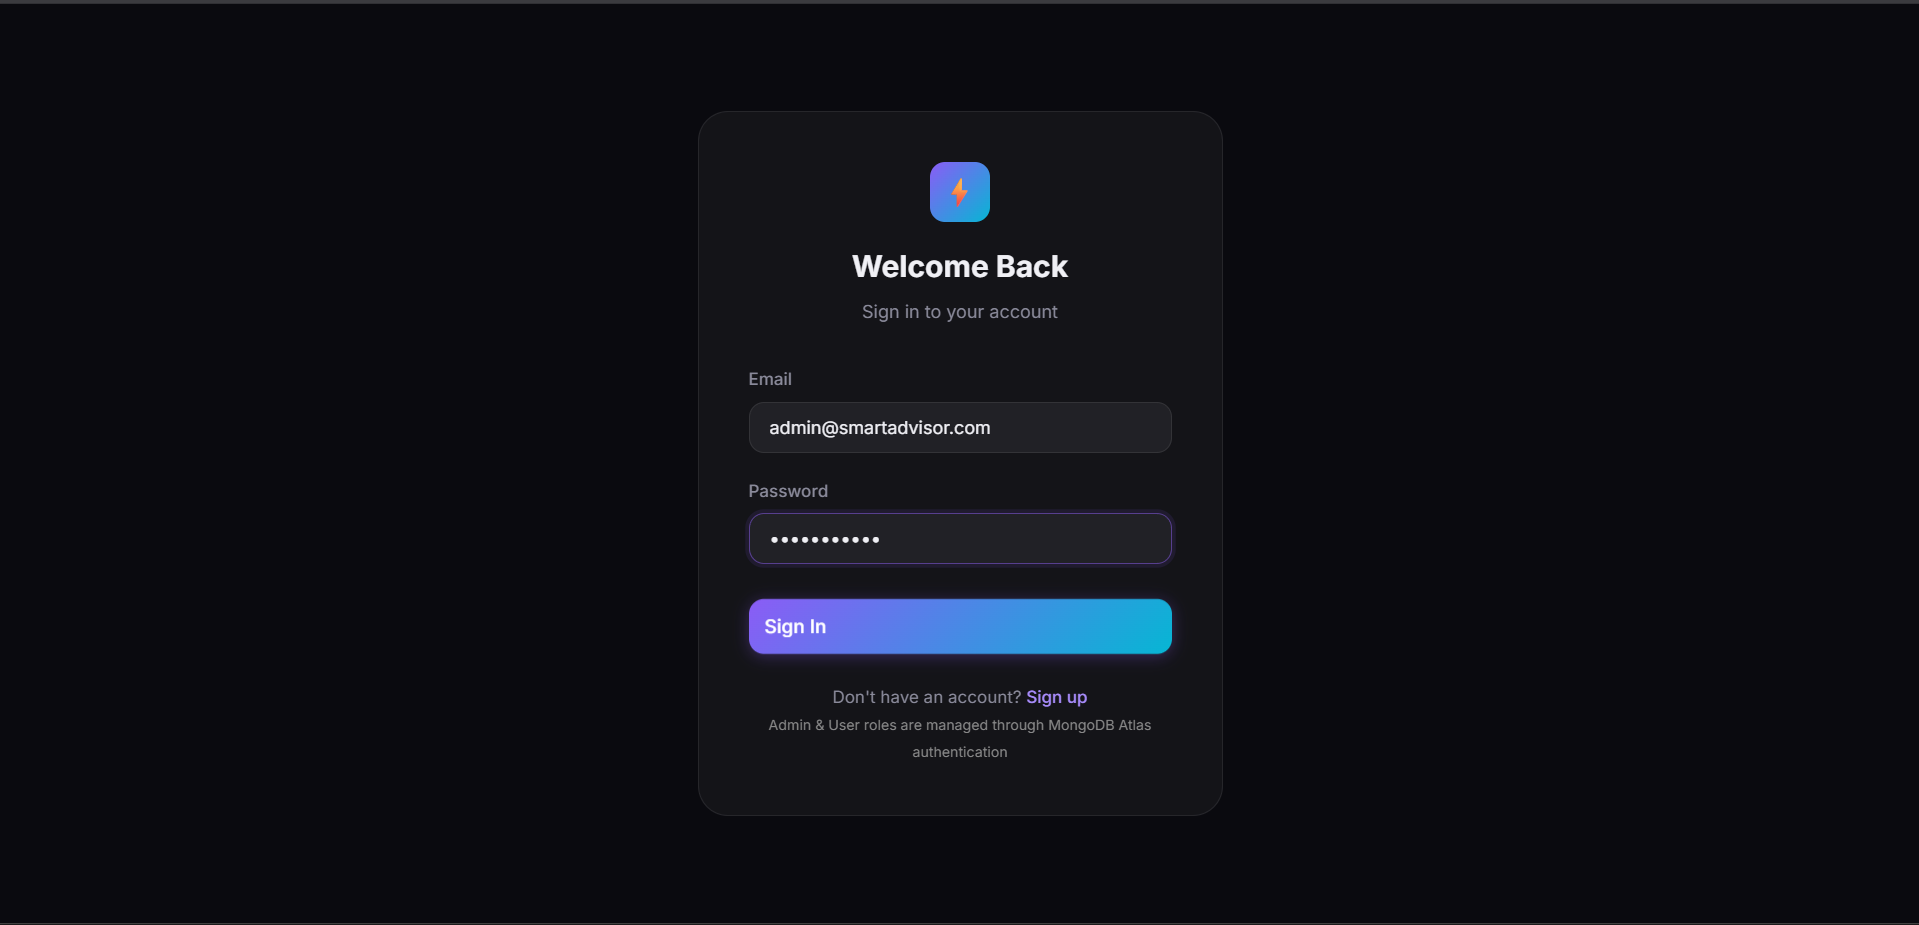
\includegraphics[width=0.85\textwidth]{image/log.png}
    \caption{Login Page}
    \label{fig:login}
\end{figure}

This screen allows users and admins to authenticate into the system securely. It validates credentials, encrypts passwords using bcrypt, and issues JWT tokens for session management.

\subsection{User Dashboard Screen}

\begin{figure}[H]
    \centering
    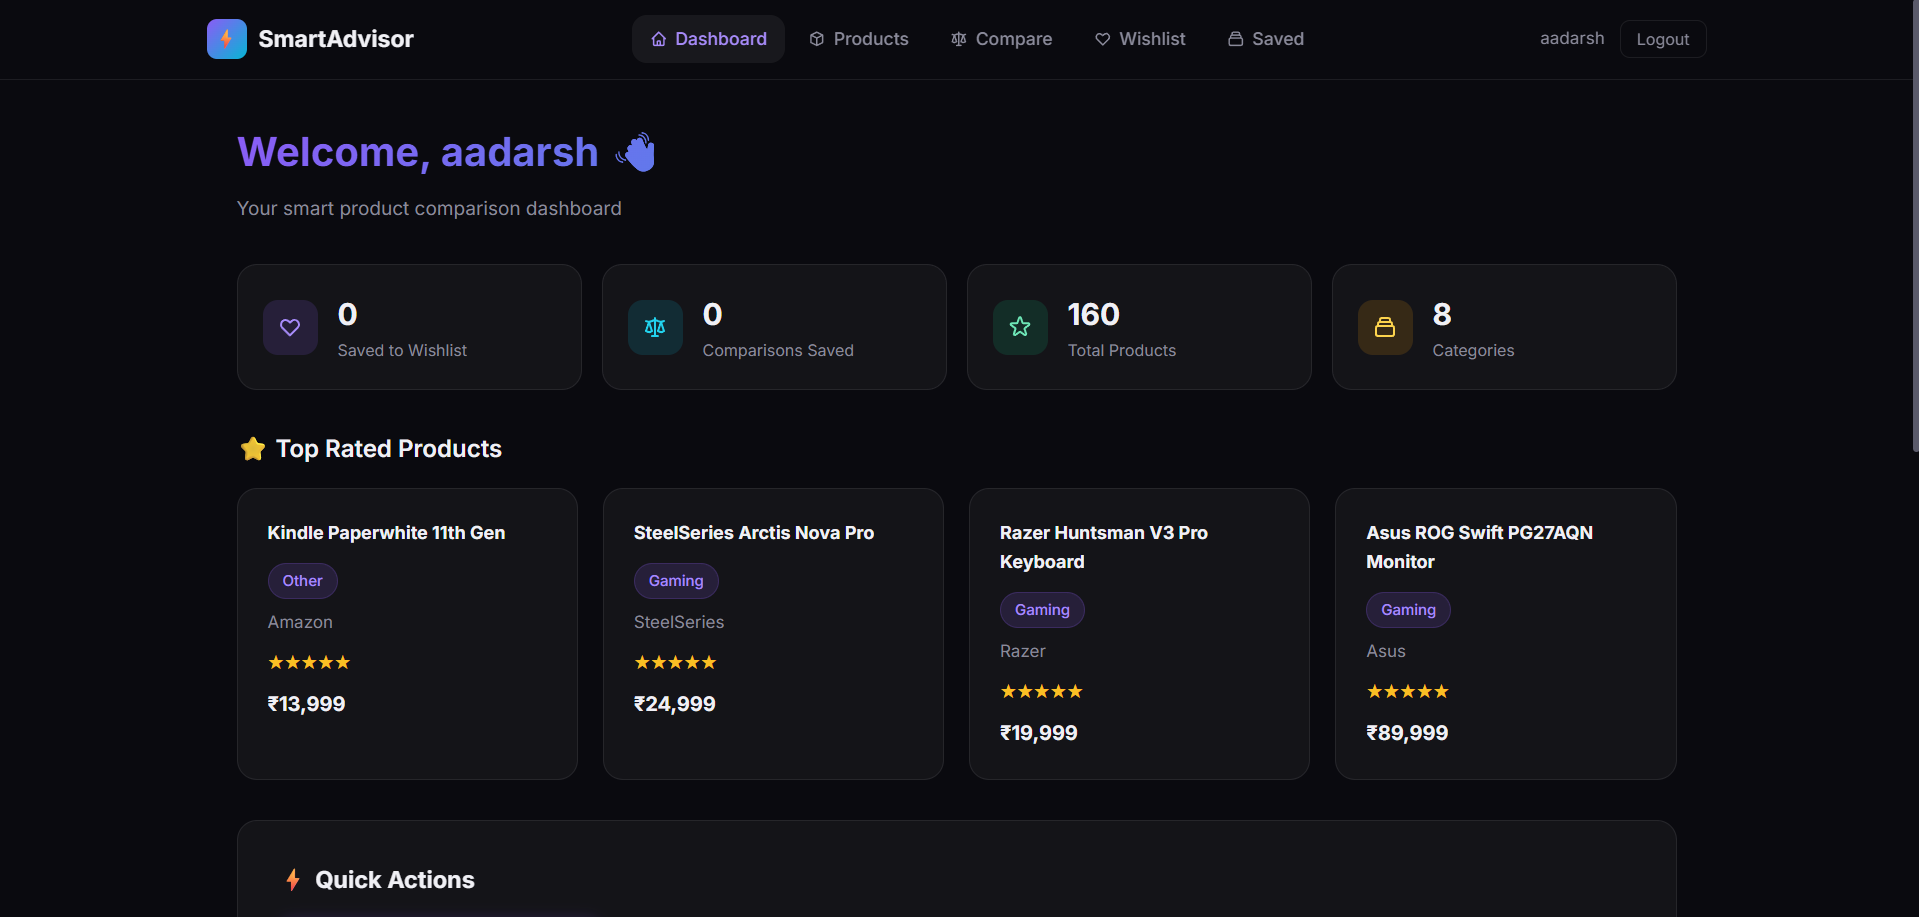
\includegraphics[width=0.85\textwidth]{image/user.png}
    \caption{User Dashboard}
    \label{fig:user_dashboard}
\end{figure}

The User Dashboard displays an overview of available products, quick access to comparison tools, and navigation to filtered product listings.

\subsection{Product Listing Screen}

\begin{figure}[H]
    \centering
    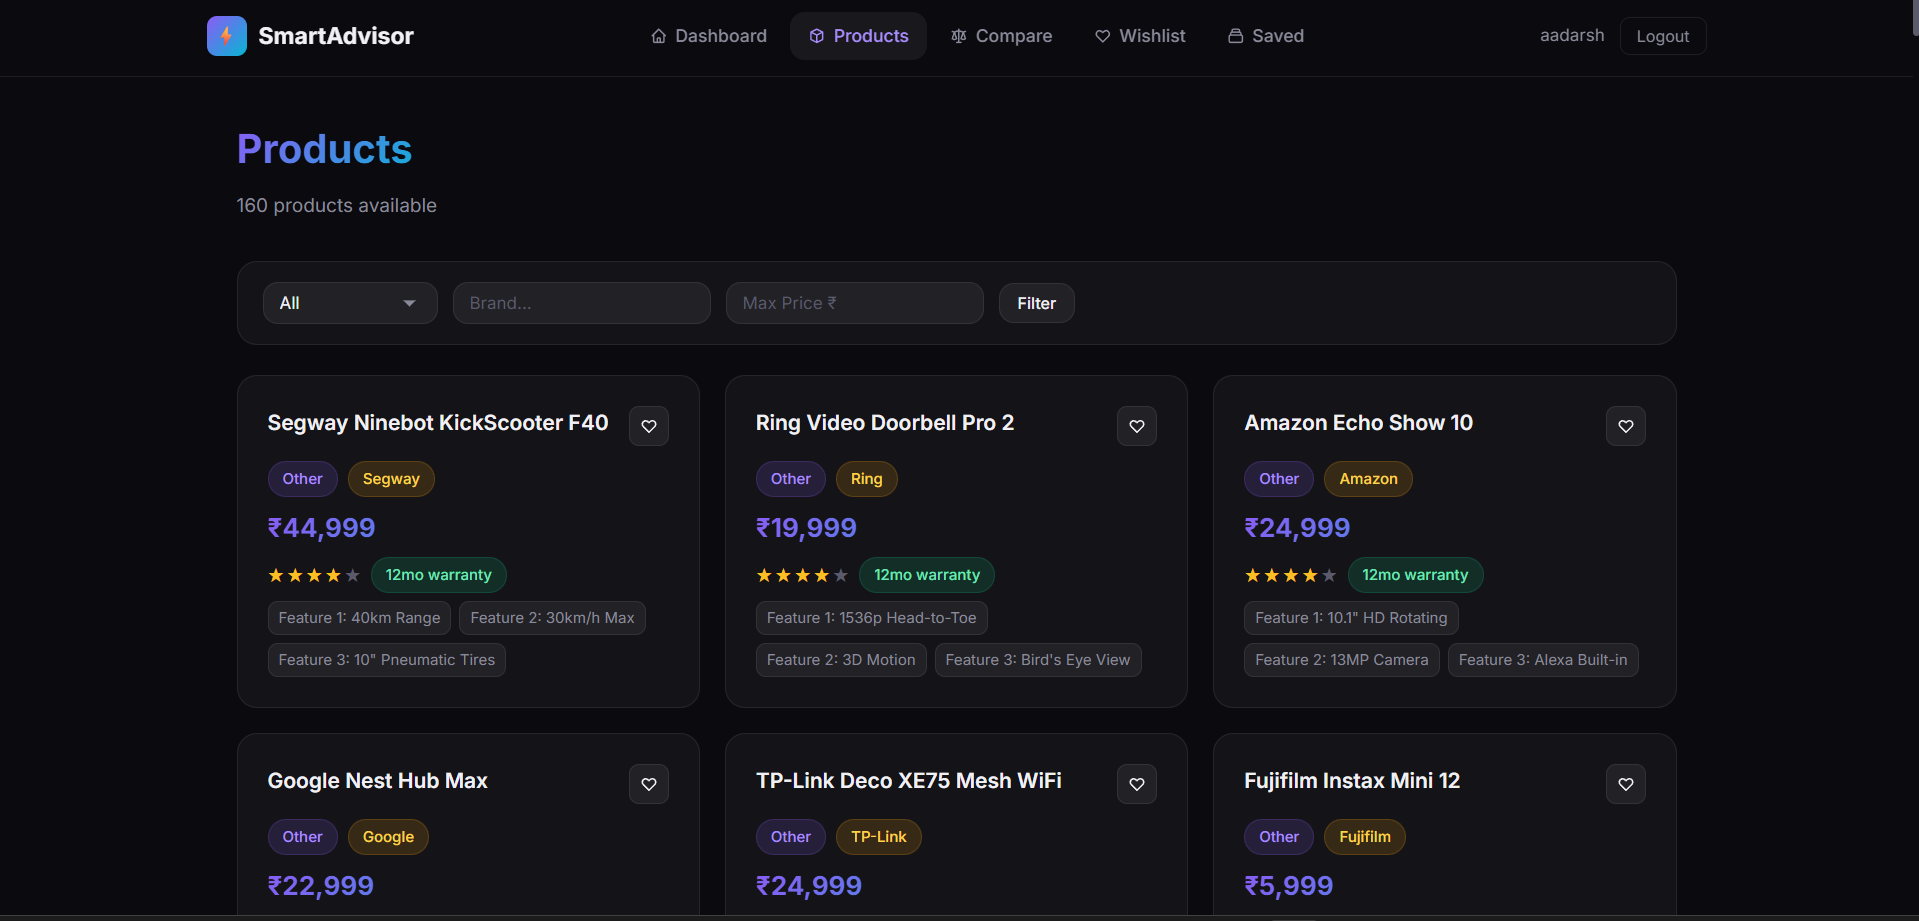
\includegraphics[width=0.85\textwidth]{image/products.png}
    \caption{Product Listing Page}
    \label{fig:products}
\end{figure}

This screen displays all available products with category filters, brand selectors, and price range options. Users can browse and select products for detailed viewing or comparison.

\subsection{Product Comparison Screen}

\begin{figure}[H]
    \centering
    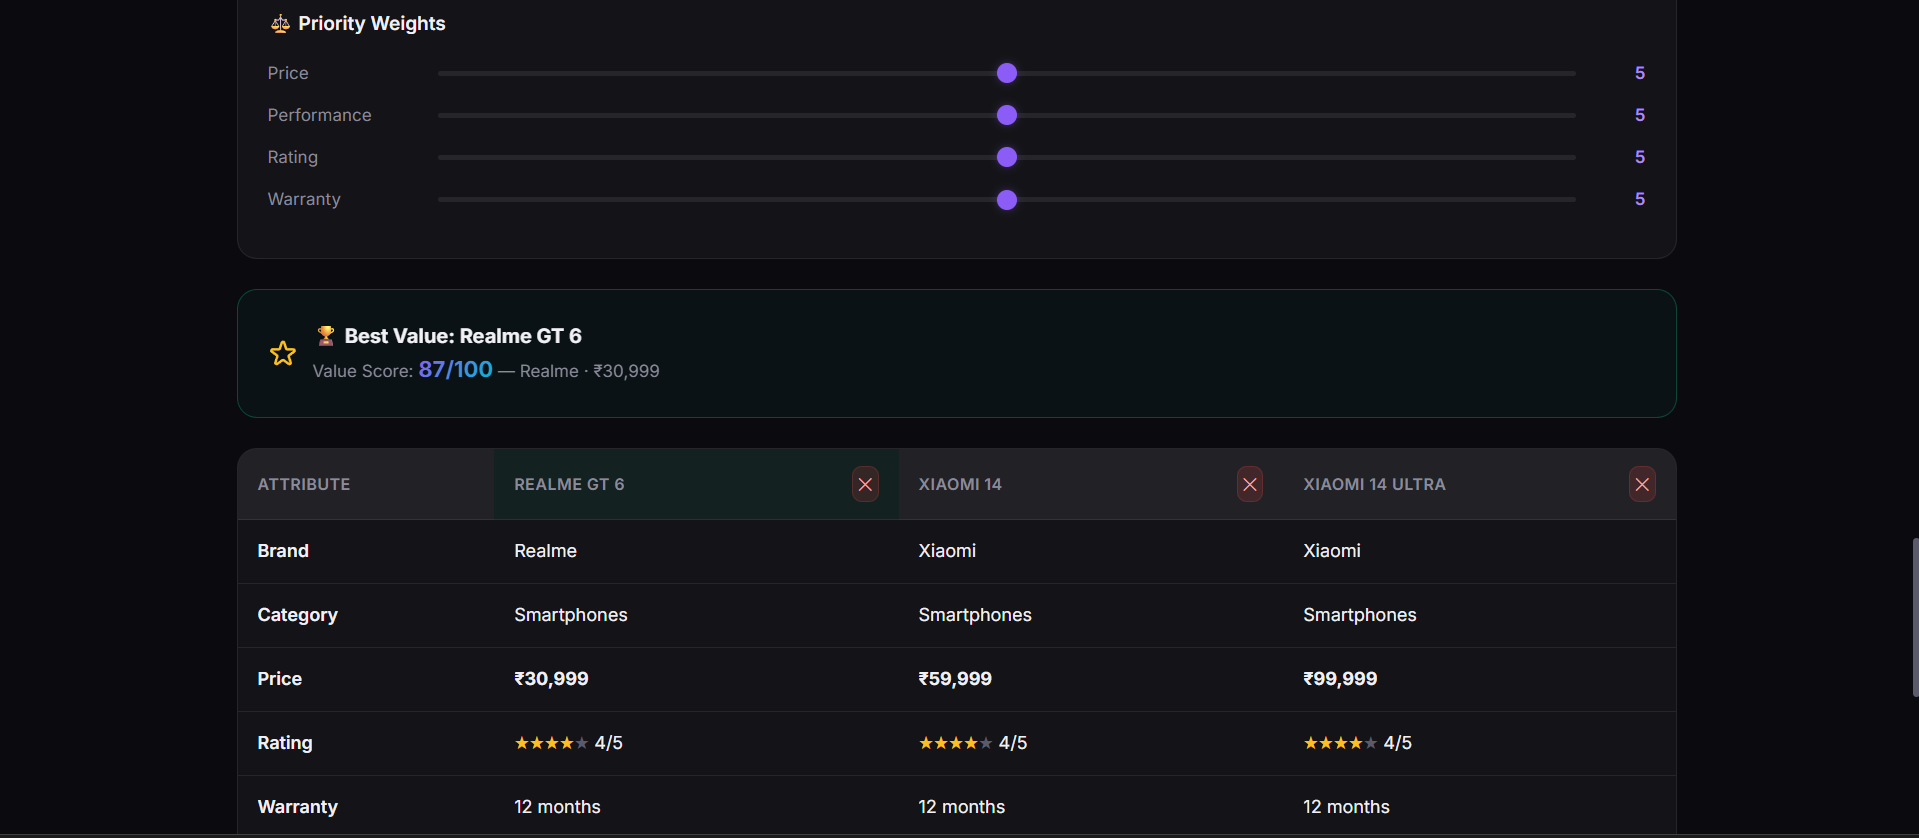
\includegraphics[width=0.85\textwidth]{image/compare.png}
    \caption{Product Comparison Page}
    \label{fig:compare}
\end{figure}

The comparison screen presents a side-by-side view of selected products, highlighting differences in specifications, ratings, price, and the calculated value score.

\subsection{Detailed Comparison View}

\begin{figure}[H]
    \centering
    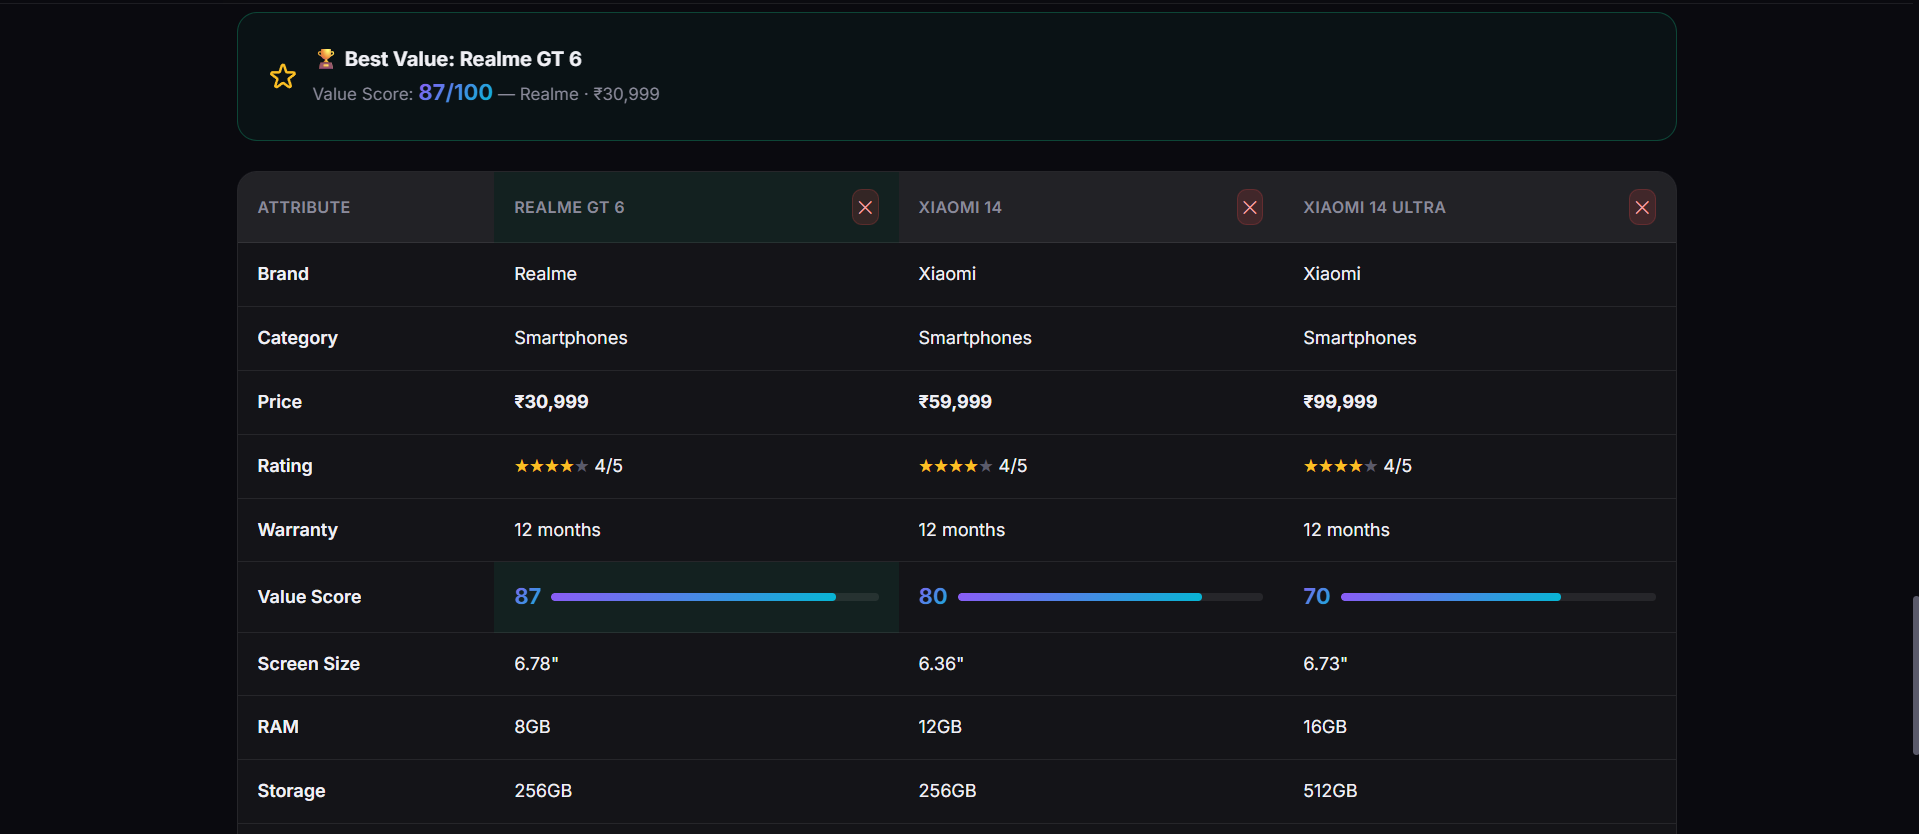
\includegraphics[width=0.85\textwidth]{image/comparison.png}
    \caption{Detailed Product Comparison View}
    \label{fig:comparison_detail}
\end{figure}

This view provides an in-depth attribute-by-attribute comparison with visual indicators to help users quickly identify the best-value product.

\subsection{Admin Dashboard Screen}

\begin{figure}[H]
    \centering
    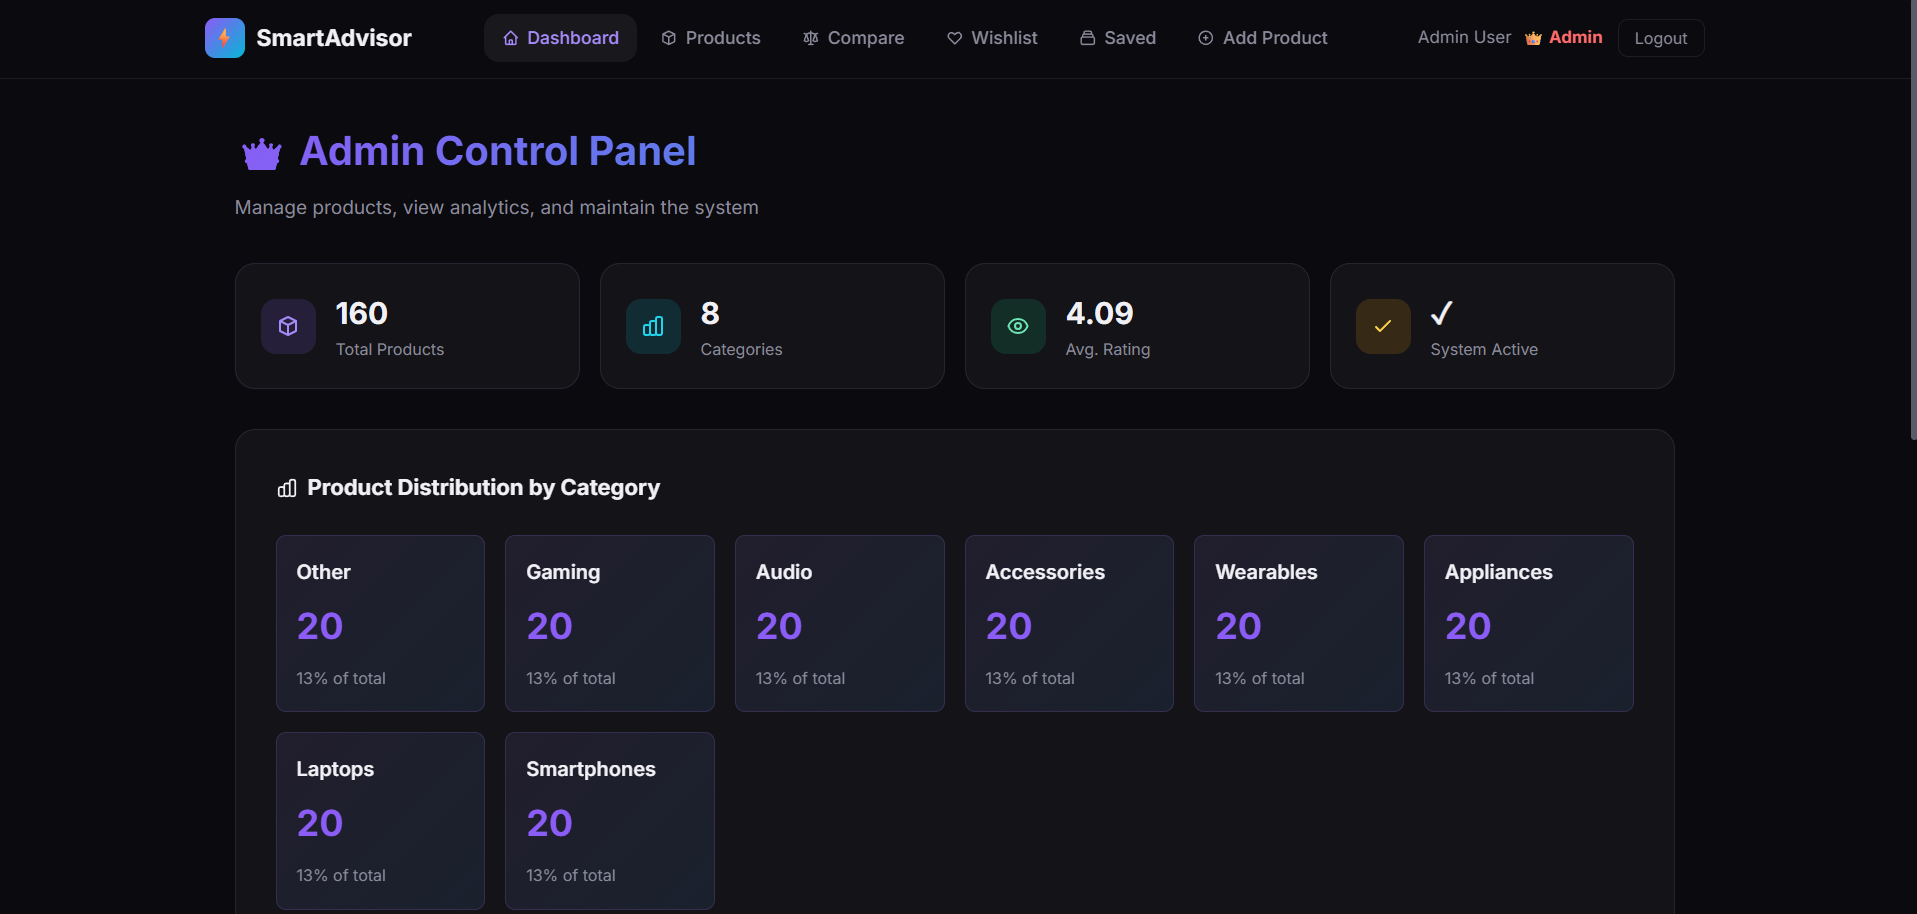
\includegraphics[width=0.85\textwidth]{image/admin dashboard.png}
    \caption{Admin Dashboard}
    \label{fig:admin_dashboard}
\end{figure}

The Admin Dashboard provides a management interface for adding, editing, and deleting products. It includes summary statistics and quick access to all administrative functions.

% =====================================================

\section{Class Diagram}

\begin{figure}[H]
    \centering
    \begin{tikzpicture}[
        class/.style={
            rectangle, draw=black!70, fill=white,
            minimum width=5cm, align=left, font=\scriptsize,
            inner sep=0pt
        },
        classname/.style={
            rectangle, draw=black!70, fill=blue!15,
            minimum width=5cm, minimum height=0.6cm,
            align=center, font=\scriptsize\bfseries,
            inner sep=3pt
        },
        classbody/.style={
            rectangle, draw=black!70, fill=white,
            minimum width=5cm, align=left, font=\scriptsize,
            inner sep=4pt, text width=4.6cm
        },
        rel/.style={-Latex, thick, black!60},
        diamond rel/.style={-{Diamond[open,length=3mm,width=2mm]}, thick, black!60}
    ]

    % ============ USER CLASS ============
    \node[classname] (user_name) at (-4, 0) {User};
    \node[classbody, anchor=north] (user_attr) at (user_name.south) {
        - name : String \\
        - email : String \\
        - password : String \\
        - role : String (user/admin) \\
        - createdAt : Date \\
        - updatedAt : Date
    };
    \node[classbody, anchor=north] (user_meth) at (user_attr.south) {
        + register() \\
        + login() \\
        + matchPassword() \\
        + logout()
    };

    % ============ PRODUCT CLASS ============
    \node[classname] (prod_name) at (4, 0) {Product};
    \node[classbody, anchor=north] (prod_attr) at (prod_name.south) {
        - name : String \\
        - category : String \\
        - brand : String \\
        - price : Number \\
        - specs : Map$\langle$String,String$\rangle$ \\
        - rating : Number \\
        - review : String \\
        - warranty : Number \\
        - userId : ObjectId$\rightarrow$User
    };
    \node[classbody, anchor=north] (prod_meth) at (prod_attr.south) {
        + addProduct() \\
        + updateProduct() \\
        + deleteProduct() \\
        + getValueScore()
    };

    % ============ COMPARISON CLASS ============
    \node[classname] (comp_name) at (-4, -6.5) {Comparison};
    \node[classbody, anchor=north] (comp_attr) at (comp_name.south) {
        - userId : ObjectId$\rightarrow$User \\
        - title : String \\
        - products : [ObjectId$\rightarrow$Product] \\
        - createdAt : Date
    };
    \node[classbody, anchor=north] (comp_meth) at (comp_attr.south) {
        + createComparison() \\
        + deleteComparison()
    };

    % ============ WISHLIST CLASS ============
    \node[classname] (wish_name) at (4, -6.5) {Wishlist};
    \node[classbody, anchor=north] (wish_attr) at (wish_name.south) {
        - userId : ObjectId$\rightarrow$User \\
        - productId : ObjectId$\rightarrow$Product \\
        - createdAt : Date
    };
    \node[classbody, anchor=north] (wish_meth) at (wish_attr.south) {
        + addToWishlist() \\
        + removeFromWishlist()
    };

    % ============ RELATIONSHIPS ============
    % User --> Product  (1 to many)
    \draw[rel] (user_attr.east) -- node[above, font=\tiny, midway] {1..*} (prod_attr.west);

    % User --> Comparison  (1 to many)
    \draw[rel] ([xshift=-0.5cm]user_meth.south) -- node[left, font=\tiny, midway] {1..*} (comp_name.north);

    % User --> Wishlist  (1 to many)
    \draw[rel] ([xshift=0.5cm]user_meth.south) -- node[right, font=\tiny, near start, xshift=0.8cm] {1..*} (wish_name.north);

    % Comparison --> Product (many to many)
    \draw[diamond rel] (comp_attr.east) -- node[above, font=\tiny, midway] {*..*} (wish_attr.west);

    % Product --> Wishlist
    \draw[rel] ([xshift=0.5cm]prod_meth.south) -- node[right, font=\tiny, midway] {0..*} (wish_name.north west);

    \end{tikzpicture}
    \caption{Class Diagram for Smart Price-to-Quality Product Advisor System}
    \label{fig:class_diagram}
\end{figure}

\textbf{Diagram Explanation}

The Class Diagram represents the structural design of the system, showing four main entity classes derived directly from the Mongoose schemas.

\textbf{User Class:} Stores user credentials with role-based differentiation (user/admin). Passwords are hashed with bcrypt. Methods include register, login, matchPassword, and logout.

\textbf{Product Class:} Holds all product information including name, category, brand, price, specs (stored as a Map), rating, review, warranty, and a reference to the admin user who created it. The getValueScore() method computes the Price-to-Quality score.

\textbf{Comparison Class:} Links a user to a set of products for side-by-side comparison. Each comparison has a title and an array of product references.

\textbf{Wishlist Class:} Provides a many-to-many relationship between users and products, allowing users to bookmark products for future reference. A unique compound index prevents duplicate entries.

% =====================================================

\section{MERN Architecture Diagram}

\begin{figure}[H]
    \centering
    \begin{tikzpicture}[
        node distance=1.5cm,
        layer/.style={rectangle, draw=black!50, rounded corners=6pt, minimum width=11cm, minimum height=1.8cm, align=center, font=\small},
        component/.style={rectangle, draw=gray!60, fill=white, rounded corners=3pt, minimum width=2.4cm, minimum height=0.7cm, align=center, font=\scriptsize},
        flow/.style={-{Stealth[length=3mm]}, thick, blue!50},
        flowback/.style={{Stealth[length=3mm]}-, thick, green!50!black}
    ]

    % ---- Client Layer ----
    \node[layer, fill=cyan!8] (client) {};
    \node[font=\small\bfseries, above] at ([yshift=-0.5cm]client.north) {Client Layer (React.js + Vite)};
    \node[component, fill=cyan!15] (login_c) at ([xshift=-3.5cm, yshift=-0.3cm]client.center) {Login / Signup};
    \node[component, fill=cyan!15] (dash_c) at ([xshift=-1cm, yshift=-0.3cm]client.center) {Dashboard};
    \node[component, fill=cyan!15] (prod_c) at ([xshift=1.5cm, yshift=-0.3cm]client.center) {Products};
    \node[component, fill=cyan!15] (comp_c) at ([xshift=3.8cm, yshift=-0.3cm]client.center) {Compare};

    % ---- API Layer ----
    \node[layer, fill=green!8, below=1.2cm of client] (api) {};
    \node[font=\small\bfseries, above] at ([yshift=-0.5cm]api.north) {API Layer (Express.js + Node.js)};
    \node[component, fill=green!12] (auth_r) at ([xshift=-3.5cm, yshift=-0.3cm]api.center) {/api/auth};
    \node[component, fill=green!12] (prod_r) at ([xshift=-1cm, yshift=-0.3cm]api.center) {/api/products};
    \node[component, fill=green!12] (comp_r) at ([xshift=1.5cm, yshift=-0.3cm]api.center) {/api/comparisons};
    \node[component, fill=green!12] (wish_r) at ([xshift=3.8cm, yshift=-0.3cm]api.center) {/api/wishlist};

    % ---- Middleware ----
    \node[layer, fill=orange!8, minimum height=1cm, below=1.2cm of api] (mid) {};
    \node[font=\small\bfseries] at ([xshift=-2.5cm]mid.center) {Middleware};
    \node[component, fill=orange!12] at ([xshift=1.5cm]mid.center) {JWT Auth + Role Check};

    % ---- Database Layer ----
    \node[layer, fill=violet!8, below=1.2cm of mid] (db) {};
    \node[font=\small\bfseries, above] at ([yshift=-0.5cm]db.north) {Database Layer (MongoDB Atlas)};
    \node[component, fill=violet!12] (user_col) at ([xshift=-3cm, yshift=-0.3cm]db.center) {Users};
    \node[component, fill=violet!12] (prod_col) at ([xshift=-0.5cm, yshift=-0.3cm]db.center) {Products};
    \node[component, fill=violet!12] (comp_col) at ([xshift=2cm, yshift=-0.3cm]db.center) {Comparisons};
    \node[component, fill=violet!12] (wish_col) at ([xshift=4cm, yshift=-0.3cm]db.center) {Wishlists};

    % ---- Arrows ----
    \draw[flow] (client.south) -- node[right, font=\tiny] {HTTP Requests} (api.north);
    \draw[flowback] (client.south) ++(0.3,0) -- ++(0,-.55) -- ([yshift=0.3cm, xshift=0.3cm]api.north) node[right, font=\tiny, midway] {JSON Responses};
    \draw[flow] (api.south) -- (mid.north);
    \draw[flow] (mid.south) -- node[right, font=\tiny] {Mongoose ODM} (db.north);

    \end{tikzpicture}
    \caption{MERN Stack Architecture Diagram}
    \label{fig:mern_arch}
\end{figure}

\textbf{Architecture Explanation:}
The frontend communicates with the backend using REST APIs. The backend processes requests through Express.js middleware (JWT authentication and role-based access control), interacts with MongoDB via Mongoose ODM, and returns JSON responses to the client.

% =====================================================

\section{Project Design}

The Smart Price-to-Quality Product Advisor System follows the MERN stack architecture:

\begin{itemize}
    \item \textbf{MongoDB} -- NoSQL document database hosted on MongoDB Atlas
    \item \textbf{Express.js} -- Backend web framework for RESTful API routing
    \item \textbf{React.js} -- Frontend library with Vite for fast builds
    \item \textbf{Node.js} -- Server-side JavaScript runtime environment
\end{itemize}

The system ensures:
\begin{itemize}
    \item Secure authentication using JWT tokens and bcrypt password hashing
    \item Efficient data retrieval through Mongoose ODM with indexed queries
    \item Scalable architecture with separated frontend and backend services
    \item Responsive user interface across desktop, tablet, and mobile devices
\end{itemize}

This structured design ensures reliability, maintainability, and future scalability.

% =====================================================

\section{Sequence Diagram}

\begin{figure}[H]
    \centering
    \begin{tikzpicture}[
        actor/.style={rectangle, draw=blue!60, fill=blue!8, minimum width=2cm, minimum height=0.6cm, align=center, font=\scriptsize\bfseries, rounded corners=2pt},
        lifeline/.style={dashed, gray!50, thick},
        msg/.style={-{Stealth[length=2.5mm]}, thick, blue!60},
        ret/.style={-{Stealth[length=2.5mm]}, thick, green!50!black, dashed},
        selfmsg/.style={-{Stealth[length=2.5mm]}, thick, orange!70},
        activation/.style={fill=blue!10, draw=blue!30, minimum width=0.35cm},
        note/.style={rectangle, draw=gray!40, fill=yellow!10, rounded corners=2pt, font=\tiny, align=left, inner sep=2pt}
    ]

    % ---- Actors ----
    \node[actor] (user) at (0, 0) {User};
    \node[actor] (react) at (3.5, 0) {React Frontend};
    \node[actor] (express) at (7.5, 0) {Express API};
    \node[actor] (mongo) at (11.5, 0) {MongoDB};

    % ---- Lifelines ----
    \draw[lifeline] (user.south) -- ++(0, -14);
    \draw[lifeline] (react.south) -- ++(0, -14);
    \draw[lifeline] (express.south) -- ++(0, -14);
    \draw[lifeline] (mongo.south) -- ++(0, -14);

    % ---- User Login Flow ----
    \node[note] at (-1.8, -0.8) {Login Flow};
    \draw[msg] (0, -1.2) -- node[above, font=\tiny] {Enter Credentials} (3.5, -1.2);
    \draw[msg] (3.5, -1.8) -- node[above, font=\tiny] {POST /api/auth/login} (7.5, -1.8);
    \draw[msg] (7.5, -2.4) -- node[above, font=\tiny] {findOne(email)} (11.5, -2.4);
    \draw[ret] (11.5, -2.9) -- node[above, font=\tiny] {User Document} (7.5, -2.9);
    \draw[selfmsg] (7.5, -3.3) -- ++(0.8, 0) -- ++(0, -0.4) -- ++(-0.8, 0) node[right, font=\tiny, xshift=0.9cm, yshift=0.2cm] {Verify bcrypt};
    \draw[ret] (7.5, -3.9) -- node[above, font=\tiny] {JWT Token} (3.5, -3.9);
    \draw[ret] (3.5, -4.4) -- node[above, font=\tiny] {Redirect to Dashboard} (0, -4.4);

    % ---- Product Comparison Flow ----
    \node[note] at (-1.8, -5.2) {Compare Flow};
    \draw[msg] (0, -5.6) -- node[above, font=\tiny] {Select Products} (3.5, -5.6);
    \draw[msg] (3.5, -6.2) -- node[above, font=\tiny] {GET /api/products?ids=...} (7.5, -6.2);
    \draw[msg] (7.5, -6.8) -- node[above, font=\tiny] {find(\{ids\})} (11.5, -6.8);
    \draw[ret] (11.5, -7.3) -- node[above, font=\tiny] {Product Documents} (7.5, -7.3);
    \draw[selfmsg] (7.5, -7.7) -- ++(0.8, 0) -- ++(0, -0.4) -- ++(-0.8, 0) node[right, font=\tiny, xshift=0.9cm, yshift=0.2cm] {Compute Scores};
    \draw[ret] (7.5, -8.3) -- node[above, font=\tiny] {Products + Value Scores} (3.5, -8.3);
    \draw[ret] (3.5, -8.8) -- node[above, font=\tiny] {Display Comparison Table} (0, -8.8);

    % ---- Admin Add Product Flow ----
    \node[note] at (-1.8, -9.6) {Admin Flow};
    \draw[msg] (0, -10) -- node[above, font=\tiny] {Submit New Product} (3.5, -10);
    \draw[msg] (3.5, -10.6) -- node[above, font=\tiny] {POST /api/products (JWT)} (7.5, -10.6);
    \draw[selfmsg] (7.5, -11) -- ++(0.8, 0) -- ++(0, -0.4) -- ++(-0.8, 0) node[right, font=\tiny, xshift=0.9cm, yshift=0.2cm] {Check Admin Role};
    \draw[msg] (7.5, -11.6) -- node[above, font=\tiny] {create(productData)} (11.5, -11.6);
    \draw[ret] (11.5, -12.1) -- node[above, font=\tiny] {Saved Product} (7.5, -12.1);
    \draw[ret] (7.5, -12.6) -- node[above, font=\tiny] {201 Created} (3.5, -12.6);
    \draw[ret] (3.5, -13.1) -- node[above, font=\tiny] {Show Success Message} (0, -13.1);

    \end{tikzpicture}
    \caption{Sequence Diagram for Smart Price-to-Quality Product Advisor System}
    \label{fig:sequence_diagram}
\end{figure}

\textbf{Diagram Explanation:}

The Sequence Diagram illustrates three key interaction flows in the system:

\begin{enumerate}
    \item \textbf{User Login Flow:} The user enters credentials on the React frontend, which sends a POST request to the Express API. The API queries MongoDB for the user document, verifies the password using bcrypt, generates a JWT token, and redirects the user to the dashboard.

    \item \textbf{Product Comparison Flow:} The user selects products for comparison. The frontend requests product data from the API, which fetches documents from MongoDB, computes the Price-to-Quality Value Scores, and returns the comparison data for display in a side-by-side table.

    \item \textbf{Admin Product Management Flow:} The admin submits a new product through the frontend. The API validates the JWT token, checks the admin role via middleware, creates the product record in MongoDB, and returns a success response.
\end{enumerate}